
\section{Statistics}

\begingroup
\def\pgfplotsmanualcurlibrary{statistics}
\tikzset{external/figure name/.add={}{statistics_}}

\begin{pgfplotslibrary}{statistics}
    A library which provides plot handlers for statistics.
\end{pgfplotslibrary}


\subsection{Box Plots}
\label{sec:boxplots}

\begingroup

\pgfkeysgetvalue{/pgfmanual/gray key prefixes}\oldgraykeyprefixes
\pgfkeys{
    /pdflinks/search key prefixes in/.add={}{,/pgfplots/boxplot/},
    /pgfmanual/gray key prefixes/.add={/pgfplots/boxplot/,}{},
}%

Box plots are visualizations for one-dimensional distributions. They provide a
fast overview over characteristics of the distribution. Box plots are
inherently one-dimensional; they only use a second axis to place multiple box
plots next to each other.

\PGFPlots{} supports two related plot handlers: |boxplot| and
|boxplot prepared|. The |boxplot| handler takes a one-dimensional sample as
input, computes the |median|, the |lower quartile|, the |upper quartile|, the
|lower whisker| and the |upper whisker|, and visualizes the result using the
|boxplot prepared| handler. The |boxplot prepared| handler expects all required
values on input and visualizes them.


\subsubsection{Prepared Box Plots and Common Options}

The |boxplot prepared| handler is discussed first; all its customizations apply
to |boxplot| as well.

\begin{plottype}[/pgfplots]{boxplot prepared=%
    \textcolor{black}{\normalfont\marg{options with {\normalfont\texttt{boxplot/}} prefix}}%
}
    A |boxplot prepared| takes a couple of key--value pairs which describe the
    required statistics and a coordinate stream of outliers on input and draws
    a box plot.
    %
\begin{codeexample}[]
\begin{tikzpicture}
\begin{axis}
    \addplot+ [
        boxplot prepared={
            lower whisker=5,
            lower quartile=7,
            median=8.5,
            upper quartile=9.5,
            upper whisker=10,
        },
    ] table [row sep=\\,y index=0] {
        data\\ 1\\ 3\\
    };
\end{axis}
\end{tikzpicture}
\end{codeexample}
    %
    \noindent The previous example shows the main idea of |boxplot prepared|:
    each required quantity has to be provided explicitly using a key--value
    syntax. The following coordinate stream can be empty; all coordinates
    inside of it are considered to be outliers. They are drawn as scatter plot.

    A box plot produces two coordinates: one which belongs to the input data
    (for example |median|) and one which is only used for drawing purposes.
    Limits will be updated for both of them. While this is clear for the axis
    which shows the input data ($x$ in this example, see also
    |draw direction|), it should be noted that limits and scaling parameters
    for the other axis will be chosen just as for any other plot. The box's
    extend is a little bit less than one unit by default (compare
    |box extend|). As a consequence, one might need to adjust either the
    limits or the scaling parameters for the remaining axis:
    %
\begin{codeexample}[]
\begin{tikzpicture}
\begin{axis}[
    y=1.5cm,
]
    \addplot+ [
        boxplot prepared={
            lower whisker=5,
            lower quartile=7,
            median=8.5,
            upper quartile=9.5,
            upper whisker=10,
        },
    ]
        table [row sep=\\,y index=0] {
        data\\ 1\\ 3\\
    };
\end{axis}
\end{tikzpicture}
\end{codeexample}
\end{plottype}

If you place multiple plots with handler |boxplot prepared| into the same axis,
they will automatically be placed next to each other by means of the default
value of |draw position|:

\begin{pgfplotskey}{boxplot/draw position=\marg{axis unit to place box} (initially 1+\textbackslash plotnumofactualtype)}
    The |draw position| key determines how to choose the position of the box
    plot, i.e.\@ the axis unit which is free to choose.

    The initial configuration places the first box plot at $y=1$ and all
    following ones at the next integer numbers.
    %
\begin{codeexample}[]
\begin{tikzpicture}
\begin{axis}
    \addplot+ [
        boxplot prepared={
            lower whisker=42, lower quartile=45,
            median=47,
            upper quartile=47.5, upper whisker=48,
        },
    ] table [row sep=\\,y index=0] { 40\\ 34\\ 56\\ };

    \addplot+ [
        boxplot prepared={
            lower whisker=36, lower quartile=39,
            median=40,
            upper quartile=41, upper whisker=43,
        },
    ]
        % no outliers:
        coordinates {};

    \addplot+ [
        boxplot prepared={
            lower whisker=41, lower quartile=44,
            median=45,
            upper quartile=46, upper whisker=47,
        },
    ] coordinates {(0,35) (0,55)};
\end{axis}
\end{tikzpicture}
\end{codeexample}
    %
    The preceding example shows three box plots in the same axis. Note that
    they have been aligned using the default setting.

    The fact that the first $N$ |boxplot| (or the equivalent
    |boxplot prepared|) are placed at the coordinates $1,2,3, \dotsc,N$ makes
    it simple to assign tick labels: either use |ytick=data| or |ytick=1,2,3|
    combined with |yticklabels|:
    %
\begin{codeexample}[]
\begin{tikzpicture}
\begin{axis}[
    ytick={1,2,3},
    yticklabels={Group A, Group B, Group C},
]
    \addplot+ [
        boxplot prepared={
            lower whisker=42, lower quartile=45,
            median=47,
            upper quartile=47.5, upper whisker=48,
        },
    ] table [row sep=\\,y index=0] { 40\\ 34\\ 56\\ };

    \addplot+[
        boxplot prepared={
            lower whisker=36, lower quartile=39,
            median=40,
            upper quartile=41, upper whisker=43,
        },
    ] coordinates {};

    \addplot+[
        boxplot prepared={
            lower whisker=41, lower quartile=44,
            median=45,
            upper quartile=46, upper whisker=47,
        },
    ] coordinates {(0,35) (0,55)};
\end{axis}
\end{tikzpicture}
\end{codeexample}

    \noindent The |draw position| may be read from some input table using
    |draw position=\thisrow|\meta{colname}. In this case, the last encountered
    data row will be used (this remark is, of course, only useful if a data
    stream is present).

    While the default choice of |draw position| hopefully covers the most
    common use cases, one can also assign a custom value to it if specific box
    plots should be placed individually:
    %
\begin{codeexample}[]
\begin{tikzpicture}
\begin{axis}[
    boxplot/draw direction=y,
]
    \addplot+ [boxplot prepared={
        lower whisker=2.5, lower quartile=4,
        median=8.5, upper quartile=12,
        upper whisker=15},
    ] coordinates {};
    \addplot+ [boxplot prepared={
        lower whisker=2.5, lower quartile=4,
        median=8.5, upper quartile=12,
        upper whisker=15},
    ] coordinates {};
    \addplot+ [boxplot prepared={draw position=5,
        lower whisker=2.5, lower quartile=4,
        median=8.5, upper quartile=12,
        upper whisker=15},
    ] coordinates {};
\end{axis}
\end{tikzpicture}
\end{codeexample}
    %
    \noindent The example shows the first two plots using the default
    |draw position|. As this uses the plot index $+1$, they are placed at $x=1$
    and $x=2$, respectively (using $x$ due to |draw direction=y|). The third
    plot has |draw position=5| and is drawn at $x=5$.

    Note that if you assign |draw position| for one plot, you may also need to
    adopt all followings ones as \PGFPlots{} does not automatically detect
    collisions.
\end{pgfplotskey}

\noindent The preceding examples read their outlier data streams from the $y$
coordinate of the input streams: for |\addplot table|, we have explicitly said
|y index=0| and for |\addplot coordinates|, we have used |(0,35) (0,55)| where
the $x$ components are ignored. This default can be changed using the
|boxplot/data| key.

\begin{pgfplotskey}{boxplot/data=\marg{expression} (initially y)}
    Tells |boxplot| how to get its data. The common idea is to provide a
    mathematical \meta{expression} which depends on data supplied by the
    |\addplot| statement. For example, if you have |\addplot expression|, the
    \meta{expression} may depend upon |x|, |y| or |z|. In case of an
    |\addplot table| input routine, the \meta{expression} can employ
    |\thisrow|\marg{colname} to access the currently active table row in the
    designated column.

    It is also possible to avoid invocations of the math parser. Use
    \declareandlabel{boxplot/data value}|=|\marg{value} instead to do so. Here,
    \meta{value} should be of a numeric constant.

    The initial configuration employs what would usually become the final |y|
    coordinate as input (to be more precise, the initial value is
    |data value=\pgfkeysvalueof{/data point/y}|).
\end{pgfplotskey}

\begin{pgfplotskey}{boxplot/data filter/.code={\marg{code}} (initially empty)}
    Allows the user to install a filter. This filter works very similarly to
    the other filters.
    %
\begin{codeexample}[]
\pgfplotsset{
    only if/.style args={entry of #1 is #2}{
        /pgfplots/boxplot/data filter/.code={
            \edef\tempa{\thisrow{#1}}
            \edef\tempb{#2}
            \ifx\tempa\tempb
            \else
                \def\pgfmathresult{}
            \fi
        }
    }
}

% 'data.dat' contains
% v     set
% 0.1   a
% 0.2   a
% 0.3   a
% 0.8   b
% 0.9   b
% 1.0   b

\begin{tikzpicture}
\begin{axis}[
    boxplot,
    table/y=v,
    boxplot/draw direction=y,
]
 \addplot table[only if={entry of set is a}]{data.dat};
 \addplot table[only if={entry of set is b}]{data.dat};
\end{axis}
\end{tikzpicture}
\end{codeexample}
\end{pgfplotskey}

\begin{pgfplotskeylist}{%
    boxplot/lower whisker=\marg{value} (initially auto),
    boxplot/lower quartile=\marg{value} (initially auto),
    boxplot/median=\marg{value} (initially auto),
    boxplot/upper quartile=\marg{value} (initially auto),
    boxplot/upper whisker=\marg{value} (initially auto),
    boxplot/average=\marg{value} (initially empty)%
}
    These keys constitute the supported statistics. Typically, a box plot uses
    each of them except for |average|.

    Any numeric value for \meta{value} will be used as is. This holds for both
    |boxplot prepared| and |boxplot|.

    An empty \meta{value} disables the respective key: its associated
    visualization will be omitted. This is the default for |average|.

    The value |auto| tells \PGFPlots{} to include the statistics in the
    automatic computation applied by |boxplot|. It is irrelevant for
    |boxplot prepared| (where it is essentially the same as an empty
    \meta{value}).

    The definition of the values is as follows. Assume that we have a given
    sample of a distribution, say $x_1,\dotsc,x_N$, and assume that the values
    are sorted, $x_1 < \dotsb < x_N$ (which is not a requirement for |boxplot|,
    by the way). For any real number $p$ with $0\le p\le1$, the
    ``$p$-quantile'' (or $p$--percentage) is defined as
        \[
            x_p :=
                \begin{cases}
                     x_{N \cdot p}
                        & \text{if $N \cdot p$ is an integer number}\\
                    \frac{1}{2} (x_{\lfloor N p \rfloor} + x_{\lceil N \cdot p \rceil})
                        & \text{if $N \cdot p$ is not an integer.}
                \end{cases}
        \]
    %FIXME : this is not as in textbooks! BUG in the computation!?

    |median| is the $0.5$-quantile of the input data: half of the points are
    less and half of the points are larger than the median.

    |lower quartile| is the $0.25$-quantile of the input data.

    |upper quartile| is the $0.75$-quartile of the input data.

    |lower whisker| is the smallest data value which is larger than
    |lower quartile|~$-1.5 \cdot \text{IQR}$ where $\text{IQR}$ is the
    ``interquartile range'', i.e.\@ the difference between |upper quartile| and
    |lower quartile|.

    |upper whisker| is the largest data value which is smaller than
    |upper quartile|~$+1.5 \cdot \text{IQR}$.

    |average| is the sample average. It is omitted by |boxplot| in its default
    configuration. Set it to |auto| to enable its auto-computation.
\end{pgfplotskeylist}

\begin{pgfplotskey}{boxplot/draw direction=\mchoice{x,y} (initially x)}
    Since |boxplot| is inherently one-dimensional, it can be visualized along
    the $x$- or the $y$-axis.

    The default configuration uses the $x$ direction as seen above.

    The alternative choice $y$ lets the boxes and their whiskers extend along
    the $y$-axis and stacks multiple box plots along the $x$-axis:
    %
    % FIXME : eliminate opacity=0 here!
\begin{codeexample}[]
\begin{tikzpicture}
\begin{axis}[
    boxplot/draw direction=y,
    x axis line style={opacity=0},
    axis x line*=bottom,
    axis y line=left,
    enlarge y limits,
    ymajorgrids,
    xtick={1,2,3},
    xticklabels={Group A, Group B, Group C},
]
    \addplot+ [
        boxplot prepared={
            lower whisker=42, lower quartile=45,
            median=47,
            upper quartile=47.5, upper whisker=48,
        },
    ] table [row sep=\\,y index=0] { 40\\ 34\\ 56\\ };

    \addplot+ [
        boxplot prepared={
            lower whisker=36, lower quartile=39,
            median=40,
            upper quartile=41, upper whisker=43,
        },
    ] coordinates {};

    \addplot+[
        boxplot prepared={
            lower whisker=41, lower quartile=44,
            median=45,
            upper quartile=46, upper whisker=47,
        },
    ] coordinates {(0,35) (0,55)};
\end{axis}
\end{tikzpicture}
\end{codeexample}
\end{pgfplotskey}

\begin{pgfplotskey}{boxplot/variable width=\mchoice{true,false} (initially false)}
    If enabled, the |box extend| will be scaled according to the |sample size|
    relative to all other |boxplot| or |boxplot prepared| within the same axis.

    The key |variable width| only has an effect if |sample size| is available.
    For |boxplot prepared|, one needs to provide |sample size| explicitly.
    %
\begin{codeexample}[]
\begin{tikzpicture}
\begin{axis}[
    ytick={1,2,3},
    yticklabels={Group A, Group B, Group C},
    boxplot/variable width,
]
    \addplot+ [% Group A:
        boxplot prepared={
            lower whisker=42, lower quartile=45,
            median=47,
            upper quartile=47.5, upper whisker=48,
            sample size=1000,
        },
    ] table [row sep=\\,y index=0] { 40\\ 34\\ 56\\ };

    \addplot+ [% Group B:
        boxplot prepared={
            lower whisker=36, lower quartile=39,
            median=40,
            upper quartile=41, upper whisker=43,
            sample size=100000,
        },
    ] coordinates {};

    \addplot+ [% Group C:
        boxplot prepared={
            lower whisker=41, lower quartile=44,
            median=45,
            upper quartile=46, upper whisker=47,
            sample size=50000,
        },
    ] coordinates {(0,35) (0,55)};
\end{axis}
\end{tikzpicture}
\end{codeexample}

    The |variable width| computation computes the largest and smallest value of
    |sample size|, chosen among all box plots in the same axis. If a single
    plot has no |sample size|, it will be omitted from the computation (and it
    will not be scaled). If a single box plot has |variable width=false|, its
    |sample size| will not contribute either. The box plot with largest value
    of |sample size| will be drawn with $100\%$ of |box extend|. The box plot
    with smallest value will be drawn with |variable width min target| times
    |box extend| as size (i.e.\@ it will receive the smallest configured size).
    All box plots in-between are scaled linearly.

    Note that the previous paragraph is not entirely true: |sample size| is
    only indirectly related to the scaling factor. Instead, the
    |variable width expr| is evaluated with the |sample size| as argument (see
    below for details).
\end{pgfplotskey}

\begin{pgfplotskey}{boxplot/sample size=\marg{number} (initially auto)}
    The number of samples used to derive the statistics. This number is used if
    |variable width=true|.

    The value \declaretext{auto} means to ``use it whenever it can be acquired
    somewhere''. For a |boxplot|, it means that the size of the input sample is
    taken as is. For a |boxplot prepared|, it means that the data is
    unavailable.

    The empty string means that the value is unavailable.

    Otherwise, a number is expected.
\end{pgfplotskey}

\begin{pgfplotskey}{boxplot/variable width expr=\marg{math expression} (initially {sqrt(\#1)})}
    A math expression which is used to evaluate the scaling factors of
    |variable width|. The argument is the current value of |sample size|. This
    key is used to implement common (nonlinear) transformations which are to be
    applied to the |sample size| before the result is used to scale down box
    sizes.

    Typically, the argument should be a monotonically increasing function.
\end{pgfplotskey}

\begin{pgfplotskeylist}{%
    boxplot/sample size min=\marg{min sample size of group} (initially empty),
    boxplot/sample size max=\marg{max sample size of group} (initially empty)%
}
    This is part of the |variable width| scaling: it is used to determine the
    |box extend| relative to all other box plots of the same group. It fixes
    the range.
\end{pgfplotskeylist}

\begin{pgfplotskey}{%
    boxplot/variable width min target=\marg{factor for the box width minimal size} (initially 0.2)%
}
    Used for the |variable width| feature to determine the size for the box
    plot with smallest value of |sample size|. The argument is interpreted to
    be a scaling factor in the range $[0,1]$.

    It is to be understood as percentage of |box extend|: a value of $1$ means
    $100\%$ of |box extend|. The initial configuration is |0.2|, meaning $20\%$
    of |box extend|.

    The box plot with largest value of |sample size| has $100\%$ of
    |box extend|.
\end{pgfplotskey}

\begin{pgfplotskey}{boxplot/box extend=\marg{axis unit for box extension} (initially 0.8)}
    A parameter which controls the size of the boxes with respect to the axis
    orthogonal to the data axis.

    The |box extend| is used as follows: if a box is centered at say, $y=1$
    with |box extend=1|, the box will start at $\nicefrac{1}{2}$ and will end at $1
    \nicefrac{1}{2}$. In other words: the box size is $1$ $y$ unit.

    It is interpreted as coordinate in the axis, and it affects the automatic
    computation of |ymin| and |ymax| values for a |boxplot|.
    %
\begin{codeexample}[]
\begin{tikzpicture}
\begin{axis}[minor y tick num=1]
    \addplot+ [
        boxplot prepared={
            lower whisker=42, lower quartile=45,
            median=47,
            upper quartile=47.5, upper whisker=48,
            box extend=1,
        },
    ] table [row sep=\\,y index=0] { 40\\ 34\\ 56\\ };

    \addplot+ [
        boxplot prepared={
            lower whisker=42, lower quartile=45,
            median=47,
            upper quartile=47.5, upper whisker=48,
            box extend=0.5, }, ]
    table [row sep=\\,y index=0] { 40\\ 34\\ 56\\ };
\end{axis}
\end{tikzpicture}
\end{codeexample}

    The |box extend| controls the size of the box and the length of the median
    line. It also controls the size of whiskers, although they have a separate
    parameter |whisker extend|.

    It is supposed to be the low-level size of a box plot, although it can be
    interpreted and used as a ``low-level variant'' of |variable width|.
\end{pgfplotskey}

\begin{pgfplotskey}{boxplot/whisker extend=\marg{axis unit for whisker extension} (initially \textbackslash pgfkeysvalueof\{/pgfplots/boxplot/box extend\}*0.8)}
    A parameter which configures how large whisker lines are with respect to
    the non-data axis.

    It is used in the same way as |box extend|, and it also affects axis
    limits.

    The initial configuration couples its value to |box extend| (it is $80\%$
    of |box extend|, to be more precise).
\end{pgfplotskey}


\begin{pgfplotskey}{boxplot/draw relative anchor=\marg{number between $0$ and $1$} (initially 0.5)}
    A key which customizes the anchor inside of the box where the whiskers are
    attached.

\begin{codeexample}[]
\begin{tikzpicture}
\begin{axis}[y=1cm]
    \addplot+ [
        boxplot prepared={
            lower whisker=42, lower quartile=45,
            median=47,
            upper quartile=47.5, upper whisker=48,
            draw relative anchor=0, }, ]
    table [row sep=\\,y index=0] { 40\\ 34\\ 56\\ };
\end{axis}
\end{tikzpicture}
\end{codeexample}

\begin{codeexample}[]
\begin{tikzpicture}
\begin{axis}[y=1cm]
    \addplot+ [
        boxplot prepared={
            lower whisker=42, lower quartile=45,
            median=47,
            upper quartile=47.5, upper whisker=48,
            draw relative anchor=0.5, }, ]
    table [row sep=\\,y index=0] { 40\\ 34\\ 56\\ };
\end{axis}
\end{tikzpicture}
\end{codeexample}

\begin{codeexample}[]
\begin{tikzpicture}
\begin{axis}[y=1cm]
    \addplot+[
        boxplot prepared={
            lower whisker=42, lower quartile=45,
            median=47,
            upper quartile=47.5, upper whisker=48,
            draw relative anchor=1, }, ]
    table [row sep=\\,y index=0] { 40\\ 34\\ 56\\ };
\end{axis}
\end{tikzpicture}
\end{codeexample}

    The value $0$ means that whisker lines are attached to the bottom of the
    box ($0\%$ of |box extend|). The value $1$ means that whisker lines are
    attached to the top edge of the box. Any value in-between is scaled
    linearly. The initial configuration is $0.5$ which means that whiskers are
    attached to the middle of the box.
\end{pgfplotskey}


\subsubsection{Analyzing Samples Automatically}

\begingroup
% this here seems to fail with gray key prefix:
\pgfkeyslet{/pgfmanual/gray key prefixes}\oldgraykeyprefixes

\begin{plottype}[/pgfplots]{boxplot=\textcolor{black}{\normalfont\marg{options with {\normalfont\texttt{boxplot/}} prefix}}}
    The |boxplot| handler takes a one-dimensional sample as input, computes the
    |median|, the |lower quartile|, the |upper quartile|, the |lower whisker|
    and the |upper whisker|, and visualizes the result using the
    |boxplot prepared| handler.

    \paragraph{Attention:}

    Computing the statistics automatically is considerably faster if you use
    |compat=1.12| combined with |lualatex|: this library has a special \lua{}
    backend which allows scalability, speed, and accuracy beyond \TeX's
    capabilities.

\begin{codeexample}[]
\begin{tikzpicture}
\begin{axis}[y=1cm]
    \addplot+ [boxplot]
        table [row sep=\\,y index=0] {
            data\\
            1\\ 2\\ 1\\ 5\\ 4\\ 10\\
            7\\ 10\\ 9\\ 8\\ 9\\ 9\\
    };
\end{axis}
\end{tikzpicture}
\end{codeexample}

    The values do not need to be sorted. However, \emph{if} they are sorted in
    ascending order, \PGFPlots{} might need less time to analyze them.

    Data points can be given by means of any supported input stream, although
    the most useful ones are probably |\addplot table| and
    |\addplot coordinates|. In any case, |boxplot| acquires only
    one-dimensional data. To this end, it uses the current value of the
    |boxplot/data| key to see which input coordinate is to be used. In the
    default configuration, this is the $y$-coordinate of the input stream. All
    other input items are ignored (except for |point meta|, which is handed
    down to the outlier stream).
\end{plottype}

\begin{pgfplotskey}{boxplot/estimator=\mchoice{value} (initially Excel)}
    Selects one of 10 available boxplot value estimators.

    The default estimator is |R7| alias |Excel| if \PGFPlots{} is configured to
    use |compat=1.12| or higher. For all older compatibility levels, it is
    |legacy|.

    The choice \declaretext{R1} resembles the estimator type 1 used by R. It
    has aliases \declaretext{SAS3} and \declaretext{Maple1}. This choice is
    currently limited to the |lua backend|.\index{lua backend required}

    The choice \declaretext{R2} resembles the estimator type 2 used by R. It
    has aliases \declaretext{SAS5} and \declaretext{Maple2}. This choice is
    currently limited to the |lua backend|.\index{lua backend required}

    The choice \declaretext{R3} resembles the estimator type 3 used by R. It
    has aliases \declaretext{SAS2}.

    The choice \declaretext{R4} resembles the estimator type 4 used by R. It
    has aliases \declaretext{SAS1}, \declaretext{SciPy0-1}, and
    \declaretext{Maple3}.

    The choice \declaretext{R5} resembles the estimator type 5 used by R. It
    has aliases \declaretext{SciPy12-12} and \declaretext{Maple4}.

    The choice \declaretext{R6} resembles the estimator type 6 used by R. It
    has aliases \declaretext{SAS4}, \declaretext{SciPy0-0}, and
    \declaretext{Maple5}.

    The choice \declaretext{R7} resembles the estimator type 7 used by R. It
    has aliases \declaretext{Excel}, \declaretext{SciPy1-1} and
    \declaretext{Maple6}.

    The choice \declaretext{R8} resembles the estimator type 8 used by R. It
    has aliases \declaretext{ScuPy13-13} and \declaretext{Maple7}.

    The choice \declaretext{R9} resembles the estimator type 9 used by R. It
    has aliases \declaretext{SciPy38-38} and \declaretext{Maple8}.

    The choice \declaretext{legacy} is a minimally repaired variant of the
    estimator which was shipped with the first version of the |statistics|
    library. It is merely kept for reasons of backwards
    compatibility.\footnote{There is also an estimator called \texttt{legacy*}.
    This is the original one shipped with the first version of this library. It
    is discouraged but kept in case someone really needs it.}
\end{pgfplotskey}

\begin{pgfplotskey}{boxplot/whisker range=\marg{number} (initially 1.5)}
    Defines how to determine |lower whisker| and |upper whisker|. In the
    default configuration, the lower whisker is placed at the smallest data
    point which is larger than |lower quartile| $- 1.5 \cdot \text{IQR}$. The
    upper whisker is placed at the largest data point which is smaller than
    |upper quartile| $+ 1.5 \cdot \text{IQR}$. Here, $\text{IQR}$ is the
    interquartile range, defined as

    $\text{IQR} := $ |upper quartile| $-$ |lower quartile|.

    Everything outside of the whisker range is supposed to be an outlier.
\end{pgfplotskey}
\endgroup


\subsubsection{Styles}

\begin{stylekey}{/pgfplots/boxplot/every boxplot}
    A style which is immediately installed whenever |boxplot| or
    |boxplot prepared| are set.

    The initial value is empty.
\end{stylekey}

\begin{stylekey}{/pgfplots/boxplot/every whisker}
    A style which is installed whenever a whisker is drawn. It is empty
    initially.
\end{stylekey}

\begin{stylekey}{/pgfplots/boxplot/every box}
    A style which is installed whenever a box is drawn. It is empty initially.
    Note that this does not apply to the path for the |median|.
\end{stylekey}

\begin{stylekey}{/pgfplots/boxplot/every median}
    A style which is installed whenever a median is drawn. It is empty
    initially.
\end{stylekey}

\begin{stylekey}{/pgfplots/boxplot/every average}
    A style which is installed whenever an average is drawn. The initial
    configuration is
    %
\begin{codeexample}[code only]
\pgfplotsset{
    boxplot/every average/.style={
        /tikz/mark=diamond*,
    },
}
\end{codeexample}
\end{stylekey}


\subsubsection{Placing Annotations}

\begin{command}{\pgfplotsboxplotvalue\marg{key name}}
    Same as

    |\pgfkeysvalueof{/pgfplots/boxplot/|\meta{key name}|}|.
\end{command}

\begin{command}{\boxplotvalue\marg{key name}}
    Same as |\pgfplotsboxplotvalue|\marg{key name} (just shorted).
\end{command}

\begin{coordinatesystem}{boxplot box}% cs=\parg{data coordinate, box-relative offset}}
   The |boxplot box cs| accepts two arguments specified a tuple of the form
   |boxplot box cs=|\parg{data coordinate, box-relative offset} where the first
   is a value of the box plot's data (it is expressed in the same space as
   |median| or |upper whisker|).

    The second argument is an offset expressed as signed multiple of
    |box extend|. An offset of $0$ means to place the point exactly on the
    bottom line of the box. An offset of $1$ places the point on the top line
    of the box. An offset of $0.5$ places the point in the middle.
    %
\begin{codeexample}[]
\begin{tikzpicture}
\begin{axis}[y=1.5cm, ymax=2]
\addplot+[boxplot]
table[row sep=\\,y index=0] {
    data\\
    1\\ 2\\ 1\\ 5\\ 4\\ 10\\
    7\\ 10\\ 9\\ 8\\ 9\\ 9\\
}
[above]
node at
  (boxplot box cs: \boxplotvalue{lower whisker},1)
  {\pgfmathprintnumber{\boxplotvalue{lower whisker}}}
node at
  (boxplot box cs: \boxplotvalue{lower quartile},1)
  {\pgfmathprintnumber{\boxplotvalue{lower quartile}}}
node[left] at
  (boxplot box cs: \boxplotvalue{median},0.5)
  {\pgfmathprintnumber{\boxplotvalue{median}}}
node at
  (boxplot box cs: \boxplotvalue{upper quartile},1)
  {\pgfmathprintnumber{\boxplotvalue{upper quartile}}}
node at
  (boxplot box cs: \boxplotvalue{upper whisker},1)
  {\pgfmathprintnumber{\boxplotvalue{upper whisker}}}
;
\end{axis}
\end{tikzpicture}
\end{codeexample}
\end{coordinatesystem}

\begin{coordinatesystem}{boxplot whisker}% cs=\parg{data coordinate, whisker-relative offset}}
    A coordinate system which is almost the same as |boxplot box cs|, except
    that it aligns at |whisker extend| instead of |box extend|.

   The |boxplot whisker cs| accepts two arguments of the form
   |boxplot whisker cs=|\parg{data coordinate, whisker-relative offset} where
   the first is a value of the box plot's data (it is expressed in the same
   space as |median| or |upper whisker|).

    The second argument is an offset expressed as signed multiple of
    |whisker extend|. An offset of $0$ means to place the point exactly on the
    lower end of the whisker line. An offset of $1$ places the point on the
    upper end of the whisker line. An offset of $0.5$ places the point in the
    middle of the whisker line.
    %
\begin{codeexample}[]
\begin{tikzpicture}
\begin{axis}[y=1.5cm, ymax=2]
\addplot+[boxplot]
table[row sep=\\,y index=0] {
    data\\
    1\\ 2\\ 1\\ 5\\ 4\\ 10\\
    7\\ 10\\ 9\\ 8\\ 9\\ 9\\
}
[above]
node at
  (boxplot whisker cs:\boxplotvalue{lower whisker},1)
  {\pgfmathprintnumber{\boxplotvalue{lower whisker}}}
node at
  (boxplot box cs: \boxplotvalue{median},1)
  {\pgfmathprintnumber{\boxplotvalue{median}}}
node at
  (boxplot whisker cs:\boxplotvalue{upper whisker},1)
  {\pgfmathprintnumber{\boxplotvalue{upper whisker}}}
;
\end{axis}
\end{tikzpicture}
\end{codeexample}
\end{coordinatesystem}

%--------------------------------------------------
% \begin{coordinatesystem}{boxplot}%
%     FIXME : is this useful? It does not respect |draw relative anchor|!
%
%     The |boxplot cs| accepts two arguments of the form
%  |boxplot cs=|\parg{data coordinate, unit offset}
%     where the first is a value of the box plot's data (just like a |median| or |upper whisker|). The second is an offset expressed in axis units. An offset of $0$ means to place the point exactly on the line which connects lower and upper whisker. A offset of $k$ adds $k$ units on top of that line, or subtracts it (if $k$ is negative).
%
%     FIXME : docs
%
% \end{coordinatesystem}
%--------------------------------------------------


\subsubsection{Customizing Visualization Paths}

The following keys are of interest if you want to redefine the shape of a box,
of a median, or of the whiskers.

Note that you should customize styles like |boxplot/every box| if you merely
wish to change fill colors.

\begin{pgfplotsxycodekeylist}{%
    boxplot/draw/lower whisker,
    boxplot/draw/upper whisker,
    boxplot/draw/whisker%
}
    A couple of code keys which customize the stroke paths for whiskers.

    The initial configuration is
    %
\begin{codeexample}[code only]
\pgfplotsset{
    boxplot/draw/lower whisker/.style={
        /pgfplots/boxplot/draw/whisker=
            {\pgfplotsboxplotvalue{lower quartile}}
            {\pgfplotsboxplotvalue{lower whisker}}
    },
    boxplot/draw/upper whisker/.style={
        /pgfplots/boxplot/draw/whisker=
            {\pgfplotsboxplotvalue{upper quartile}}
            {\pgfplotsboxplotvalue{upper whisker}}
    },
    boxplot/draw/whisker/.code 2 args={
        \draw [/pgfplots/boxplot/every whisker/.try]
            (boxplot cs:#1) -- (boxplot cs:#2)
            (boxplot whisker cs:#2,0)
            --
            (boxplot whisker cs:#2,1)
        ;
    },
}
\end{codeexample}

    The key |draw/lower whisker| key is used if and only if |lower whisker| has
    a numeric value. The key |draw/upper whisker| is used if and only if
    |upper whisker| has a value.

    If one of |lower quartile| or |upper quartile| is empty, both are replaced
    by the following values:

    |lower quartile| $:=$ |upper whisker| and

    |upper quartile| $:=$ |lower whisker|.

    Thus, if the box cannot be drawn but you only have whiskers, the two
    whiskers will be connected with each other.
\end{pgfplotsxycodekeylist}

\begin{pgfplotscodekey}{boxplot/draw/box}
    A path which is used for |every box|.
\begin{codeexample}[code only]
\pgfplotsset{
    boxplot/draw/box/.code={
        \draw [/pgfplots/boxplot/every box/.try]
            (boxplot box cs:\pgfplotsboxplotvalue{lower quartile},0)
            rectangle
            (boxplot box cs:\pgfplotsboxplotvalue{upper quartile},1)
        ;
    },
}
\end{codeexample}

    It either |lower quartile| or |upper quartile| is empty, this key will not
    be invoked.

    Note that |draw/median| will be invoked after this key.
\end{pgfplotscodekey}

\begin{pgfplotscodekey}{boxplot/draw/median}
    A path which is used for every |median|. Its initial configuration is
    %
\begin{codeexample}[code only]
\pgfplotsset{
    boxplot/draw/median/.code={
        \draw [/pgfplots/boxplot/every median/.try]
            (boxplot box cs:\pgfplotsboxplotvalue{median},0)
            --
            (boxplot box cs:\pgfplotsboxplotvalue{median},1)
        ;
    },
}
\end{codeexample}
    %
    This key will be omitted if |median| is empty.
\end{pgfplotscodekey}

\begin{pgfplotscodekey}{boxplot/draw/average}
    The path which is used to visualize an |average|. The initial configuration is
\begin{codeexample}[code only]
\makeatletter
\pgfplotsset{
    boxplot/draw/average/.code={
        \draw [/pgfplots/boxplot/every average/.try]
            \pgfextra
            % do NOT use \draw[mark=*] plot coordinates because
            % boxplots uses the same plot handler to draw its
            % outliers.
            \pgftransformshift{%
                % basic level access to 'boxplot box cs':
                \pgfplotsboxplotpointabbox
                    {\pgfplotsboxplotvalue{average}}
                    {0.5}%
            }%
            \pgfuseplotmark{\tikz@plot@mark}%
            \endpgfextra
        ;
    },
}
\makeatother
\end{codeexample}
    This key will be omitted if |average| has an empty value (the default).

    The key |draw/average| will be evaluated after |draw/median| and after
    |draw/box|.
\end{pgfplotscodekey}

\endgroup


\subsection{Histograms}
\label{sec:histograms}

\begin{plottype}[/pgfplots]{hist=\textcolor{black}{\normalfont\marg{%
        options with {\normalfont\texttt{hist/}} prefix}}%
}
    A histogram plot takes one-dimensional input data and counts the occurrence
    of values: it determines the data range $[\underline m,\overline m]$ and
    subdivides it into $N$ equally sized bins with $(N+1)$ endpoints. Then, it
    counts the number of points falling into each bin. More precisely, it
    computes the $N+1$ points $\underline m =: x_0 < x_1 < \dotsb < x_N :=
    \overline m$ using $x_i := \underline m + i \cdot (\overline m - \underline
    m)/N$. Then, it creates the $N+1$ coordinates $(x_i, y_i)$,
    $i=0,\dotsc,N-1$ by means of
    %
        \[
            y_i :=
                \begin{cases}
                    \text{bincount}\bigl([x_i,x_{i+1})\bigr)        & i < N \\
                    y_{N-1}                                         & i = N,
                \end{cases}
        \]
    %
    i.e.\@ the value of the last coordinate is replicated. This set of $(N+1)$
    interval boundaries is then visualized by an |ybar interval| plot handler.
    %
\begin{codeexample}[]
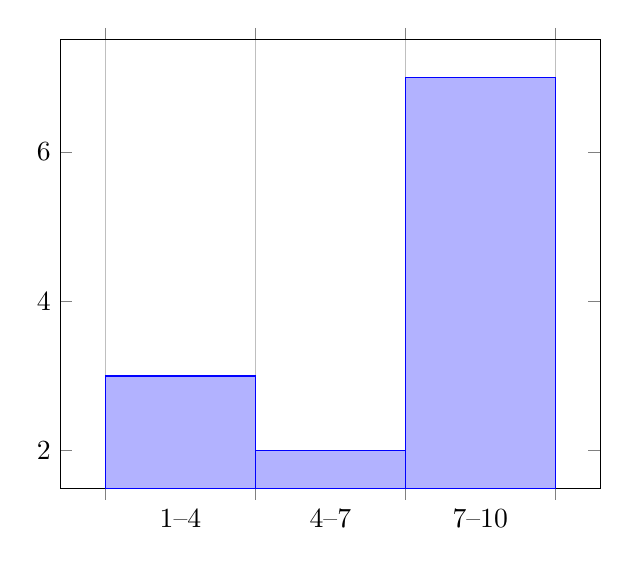
\begin{tikzpicture}
\begin{axis}[
    ybar interval,
    xticklabel=
\pgfmathprintnumber\tick--\pgfmathprintnumber\nexttick
]
    \addplot+ [hist={bins=3}]
        table [row sep=\\,y index=0] {
            data\\
            1\\ 2\\ 1\\ 5\\ 4\\ 10\\
            7\\ 10\\ 9\\ 8\\ 9\\ 9\\
    };
\end{axis}
\end{tikzpicture}
\end{codeexample}
    %
    We see that |hist={bins=3}| takes a table with one column as input. The
    data values fall into the range $[1,10]$ which is partitioned into~$3$
    intervals (of equal lengths). Finally, the number of points falling into
    each of the three bins is plotted. The |xticklabel| key shows the range
    (note that it works only in conjunction with |x tick label as interval|
    which has been enabled by |ybar interval| before). We see that there are
    $3$ elements in the range $[1,4)$, $2$~elements in the range $[4,7)$ and
    finally $7$ elements in the range $[7,10]$.

    The bins are half-open intervals, i.e.\@ the endpoint does not belong to
    the bin. Only the last bin contains its right end point.
    %
\pgfplotsexpensiveexample
\begin{codeexample}[]
\begin{tikzpicture}
\begin{axis}[
    ybar interval,
    xtick=,% reset from ybar interval
    xticklabel={
        $[\pgfmathprintnumber\tick,
         \pgfmathprintnumber\nexttick)$
    },
    x tick label style={draw=red},
]
    % a data file containing 8000 normally distributed
    % random numbers of mean 0 and variance 1
    \addplot+ [hist={data=x}]
        file {plotdata/pgfplots.randn.dat};
\end{axis}
\end{tikzpicture}
\end{codeexample}

    The |hist| plot type can be combined with \verbpdfref{plot expression} as
    well: provide the usual \meta{expression} as you would for a line plot.
    Then, configure the value for |data=|\meta{expression} in dependence of
    |x|, |y|, or |z|:
    %
\pgfplotsexpensiveexample
\begin{codeexample}[]
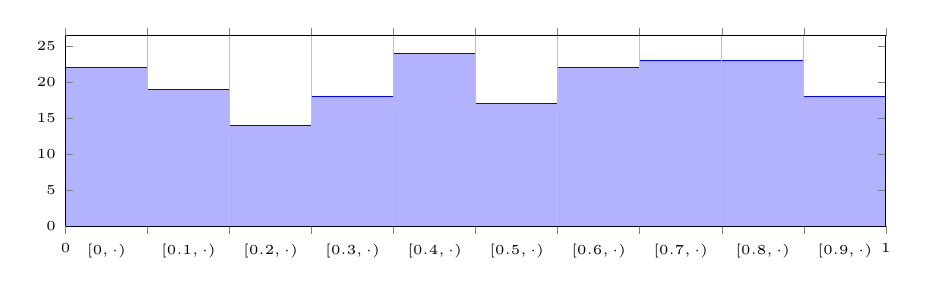
\begin{tikzpicture}
    \begin{axis}[
        tiny,
        height=4cm,width=12cm,
        ybar interval,
        ymin=0,
        xmin=0,xmax=1,
        axis on top,
        extra x ticks={0,1},
        extra x tick style={
            grid=none,
            x tick label as interval=false,
            xticklabel={$\pgfmathprintnumber\tick$}
        },
        xticklabel={$[\pgfmathprintnumber[fixed]\tick,\cdot)$},
    ]
        \addplot+ [samples=200,hist] {rnd};
    \end{axis}
\end{tikzpicture}
\end{codeexample}
    %
    \noindent The example uses the |rnd| method of \pgfname{} which defines |y|
    to contain uniform random numbers in the range $[0,1]$. Then, it configures
    |hist|. Note that |hist| has the default |data=y| such that it uses the |y|
    coordinate as input. Note furthermore that the |x| value is effectively
    ignored here. The options after |\begin{axis}[...]| are mainly to scale the
    graphics and to insert the right limits. The |extra x ticks| method is
    inserted to demonstrate how to add further tick marks without affecting the
    overall layout. Note that the |extra x tick style| sets
    |x tick label as interval=false| to disable the special tick handling which
    is active for the rest of the plot.

    The following keys configure |hist|. If they are provided inside of
    \meta{options}, the common key prefix |hist/| can be omitted.

    \begin{pgfplotskey}{hist/data=\marg{expression} (initially y)}
        Tells |hist| how to get its data. The common idea is to provide a
        mathematical \meta{expression} which depends on data supplied by the
        |\addplot| statement. For example, if you have |\addplot expression|,
        the \meta{expression} may depend upon |x|, |y| or |z|. In case of an
        |\addplot table| input routine, the \meta{expression} can employ
        |\thisrow|\marg{colname} to access the currently active table row in
        the designated column.

        It is also possible to avoid invocations of the math parser. Use
        \declareandlabel{hist/data value}|=|\marg{value} instead to do so.
        Here, \meta{value} should be of a numeric constant.

        The initial configuration employs what would usually become the final
        |y| coordinate as input (to be more precise, the initial value is
        |data value=\pgfkeysvalueof{/data point/y}|).
    \end{pgfplotskey}

    \begin{pgfplotskeylist}{%
        hist/data min=\marg{min value} (initially /pgfplots/xmin),
        hist/data max=\marg{max value} (initially /pgfplots/xmax)%
    }
        Allows to provide the min/max values (the $\underline m$ and $\overline
        m$) values manually.

        If empty, these values will be deduced from the input data range.

        The resulting interval will be split into |hist/bins| intervals.

        The initial configuration uses any provided data limits, i.e.\@ the
        (natural) choices |hist/data min=||xmin| and |hist/data max=||xmax|.
    \end{pgfplotskeylist}

    \begin{pgfplotskey}{hist/bins=\marg{number of intervals} (initially 10)}
        Specifies the number of intervals to use.
    \end{pgfplotskey}

    \begin{pgfplotskey}{hist/intervals=\marg{true,false} (initially true)}
        If |intervals=true| (the initial configuration), |hist| will generate
        $N+1$ coordinates, with
        %
            \[
                \underline m = x_0 < x_1 < \dotsb < x_{N} = \overline m
            \]
        %
        where $[\underline m,\overline m]$ is the data range. In this case, the
        data points for $x_{N-1}$ and $x_N$ will get the same value, namely the
        number of elements in the last bin. This is (only) useful in
        conjunction with |const plot| or |ybar interval|.

        If |intervals=false|, the last data point will be omitted and exactly
        $N$ coordinates will be generated. In this case, the right end point is
        not returned explicitly.
    \end{pgfplotskey}

    \begin{pgfplotskey}{hist/cumulative=\marg{true,false} (initially false)}
        Allows to compute a cumulative histogram.

        A cumulative histogram uses the sum of all previous bins and the
        current one as final value.

        Here is the example from above, this time with |hist/cumulative|:
        %
\pgfplotsexpensiveexample
\begin{codeexample}[]
\begin{tikzpicture}
\begin{axis}[
    ybar interval,
    xtick=,% reset from ybar interval
    xticklabel={
        $[\pgfmathprintnumber\tick,
        \pgfmathprintnumber\nexttick)$
    },
]
    % a data file containing 8000 normally distributed
    % random numbers of mean 0 and variance 1
    \addplot+ [hist={data=x,cumulative}]
        file {plotdata/pgfplots.randn.dat};
\end{axis}
\end{tikzpicture}
\end{codeexample}
    \end{pgfplotskey}

    \begin{pgfplotskey}{hist/density=\marg{true,false} (initially false)}
        \textit{An extension by Jürnjakob Dugge}
        \vskip\baselineskip
        Enables density estimation mode. If |hist/density| is active, the
        resulting data points will be renormalized such that the overall
        ``mass'' equals~$1$.
        %
\pgfplotsexpensiveexample
\begin{codeexample}[]
\begin{tikzpicture}
    \begin{axis}[small,ymin=0,title=\texttt{hist}]
        \addplot [
            hist,
            fill=orange!75,
            draw=orange!50!black]
                table [y index=0] {plotdata/pgfplots.randn.dat};
    \end{axis}
\end{tikzpicture}
%
\begin{tikzpicture}
    \begin{axis}[small,ymin=0, title=\texttt{hist=density}]
        \addplot [
            hist=density,
            fill=orange!75,
            draw=orange!50!black]
                table [y index=0] {plotdata/pgfplots.randn.dat};
    \end{axis}
\end{tikzpicture}
\end{codeexample}


        The keys |hist/density| and |hist/cumulative| can be combined as well:
        %
\pgfplotsexpensiveexample
\begin{codeexample}[]
\begin{tikzpicture}
    \begin{axis}[small,ymin=0, title=\texttt{hist=cumulative}]
        \addplot [
            hist=cumulative,
            fill=orange!75,
            draw=orange!50!black]
                table [y index=0] {plotdata/pgfplots.randn.dat};
    \end{axis}
\end{tikzpicture}
%
\begin{tikzpicture}
    \begin{axis}[small,ymin=0, title=\texttt{hist=\{cumulative,density\}}]
        \addplot [
            hist={cumulative,density},
            fill=orange!75,
            draw=orange!50!black]
                table [y index=0] {plotdata/pgfplots.randn.dat};
    \end{axis}
\end{tikzpicture}
\end{codeexample}
    \end{pgfplotskey}

    \begin{stylekey}{/pgfplots/hist/handler (initially ybar interval)}
        Allows to change the way the generated coordinates are visualized. The
        |hist/handler| key is a style, so use
        |hist/handler/.style={const plot}| to change it.
        %
\begin{codeexample}[]
\begin{tikzpicture}
\begin{axis}
    \addplot+ [
        hist={bins=3},
    ] table [row sep=\\,y index=0] {
        data\\
        1\\ 2\\ 1\\ 5\\ 4\\ 10\\
        7\\ 10\\ 9\\ 8\\ 9\\ 9\\
    };
\end{axis}
\end{tikzpicture}
\end{codeexample}

\begin{codeexample}[]
\begin{tikzpicture}
\begin{axis}
    \addplot+ [
        hist={
            bins=3,
            handler/.style={const plot},
        },
    ] table [row sep=\\,y index=0] {
        data\\
        1\\ 2\\ 1\\ 5\\ 4\\ 10\\
        7\\ 10\\ 9\\ 8\\ 9\\ 9\\
    };
\end{axis}
\end{tikzpicture}
\end{codeexample}

\begin{codeexample}[]
\begin{tikzpicture}
\begin{axis}
    \addplot+ [
        hist={
            bins=3,
            handler/.style={sharp plot},
        },
    ] table [row sep=\\,y index=0] {
        data\\
        1\\ 2\\ 1\\ 5\\ 4\\ 10\\
        7\\ 10\\ 9\\ 8\\ 9\\ 9\\
    };
\end{axis}
\end{tikzpicture}
\end{codeexample}

        Note that |sharp plot| might benefit from |intervals=false|:
        %
\begin{codeexample}[]
\begin{tikzpicture}
\begin{axis}
    \addplot+ [
        hist={
            bins=3,
            handler/.style={sharp plot},
            intervals=false,
        },
    ] table [row sep=\\,y index=0] {
        data\\
        1\\ 2\\ 1\\ 5\\ 4\\ 10\\
        7\\ 10\\ 9\\ 8\\ 9\\ 9\\
    };
\end{axis}
\end{tikzpicture}
\end{codeexample}
    \end{stylekey}

    \begin{pgfplotscodekey}{hist/data filter}
        Allows to define coordinate filters, similar to the coordinate filter
        key |x filter| described in Section~\ref{sec:filters}. The argument
        |#1| is the coordinate as it has been found after processing
        |hist/data|. The code is supposed to assign |\pgfmathresult| to contain
        the result. If |\pgfmathresult| is empty afterwards, it will be
        skipped. Otherwise, it is supposed to contain a number.

        This filter is applied \emph{before} the histogram is computed. Note
        that |x filter| and |y filter| are applied \emph{after} the histogram
        is computed.

        Note that predefined styles like |each nth point| can also be applied
        to |hist/data| if
        %
        \begin{enumerate}
            \item an asterisk `|*|' is appended to the predefined style's
                name and
            \item the first argument to the style is |hist/data|.
        \end{enumerate}
        %
        For example, |each nth point*={hist/data}{2}| will skip each second
        input value of |hist/data| (try it out).
    \end{pgfplotscodekey}

    \begin{pgfplotsxycodekeylist}{%
        /pgfplots/hist/data coord trafo,
        /pgfplots/hist/data coord inv trafo%
    }
        These keys work in the same way as for |x coord trafo| and
        |x coord inv trafo|. They are applied to the |hist/data| value before
        the histogram is evaluated and after the result value is assigned,
        respectively.

        Note that |hist| will apply the |hist/data coord inv trafo| before it
        visualizes its results. Consequently, it may be necessary to assign a
        similar transformation to |x coord trafo| as well.

        See the documentation of |x coord trafo| for more information about
        custom transformations.
    \end{pgfplotsxycodekeylist}

    \begin{pgfplotskey}{hist/symbolic coords=\marg{list}}
        A style which enables |symbolic x coords| for an axis containing |hist|
        plots:
        %
\begin{codeexample}[]
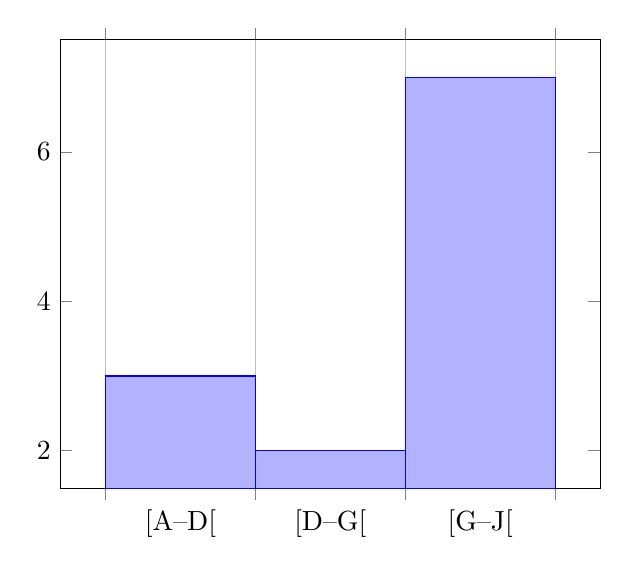
\begin{tikzpicture}
\begin{axis}[
    ybar interval,
    hist/symbolic coords={A,B,C,D,E,F,G,H,I,J},
    xticklabel={[\tick--\nexttick[},
]
    \addplot+ [
        hist={bins=3},
    ] table [row sep=\\,y index=0] {
        data\\
        A\\ B\\ A\\ D\\ F\\ J\\
        G\\ J\\ I\\ H\\ I\\ I\\
    };
\end{axis}
\end{tikzpicture}
\end{codeexample}
        %
        The style does two things: first, it defines |hist/data coord trafo|
        and |hist/data coord inv trafo|, then, it calls |symbolic x coords|
        with the same argument.


        \paragraph{Attention:}

        do not use |hist/data=x| or other symbolic values as input when you
        have |symbolic coords|. Rather than symbolic values, you need to
        provide \emph{expandable} values like |\pgfkeysvalueof{/data point/x}|
        (which has the same effect, but directly expands to the correct value).

        Please refer to the documentation of |symbolic x coords| for further
        details about symbolic coordinates.
    \end{pgfplotskey}
\end{plottype}
\endgroup
